\documentclass[aspectratio=169]{beamer}

\usetheme{vega}

% Please, avoid using more than 2 lines in the title.
% If needed, see line 178 in 'beamerthemevega.sty' to modify the vertical indentation
\title{Ценообразование и хеджирование
Автоколла}
\subtitle{Летний научный выезд Фонда "Институт "Вега"}
\author{Владимир Шин, Дарья Юневич}
\institute{Vega Institute Foundation}
\supervisor{Еркин Китапбаев, Владимир Шангин}
\date{24 июля 2023г}

\addbibresource{refs.bib}
\usepackage[]{lipsum}
\usepackage[russian]{babel}
\begin{document}
    \maketitle
    
    \begin{frame}
    \frametitle{Содержание} 
    \tableofcontents 
    \end{frame}


\section{Введение}
    \begin{frame}{Введение}
    В данной исследовательской работе:
    \newline
    \newline
    $\bullet$ Рассматривается структурный продукт, имеющий большой спрос со стороны инвесторов 

    
    $\bullet$ С помощью векторизации достигнуто ускорение вычисления ошибки дельта-хеджирования в 5 раз
  
    \end{frame}

   

\begin{frame}{Cхема выплат продукта}
\begin{center}
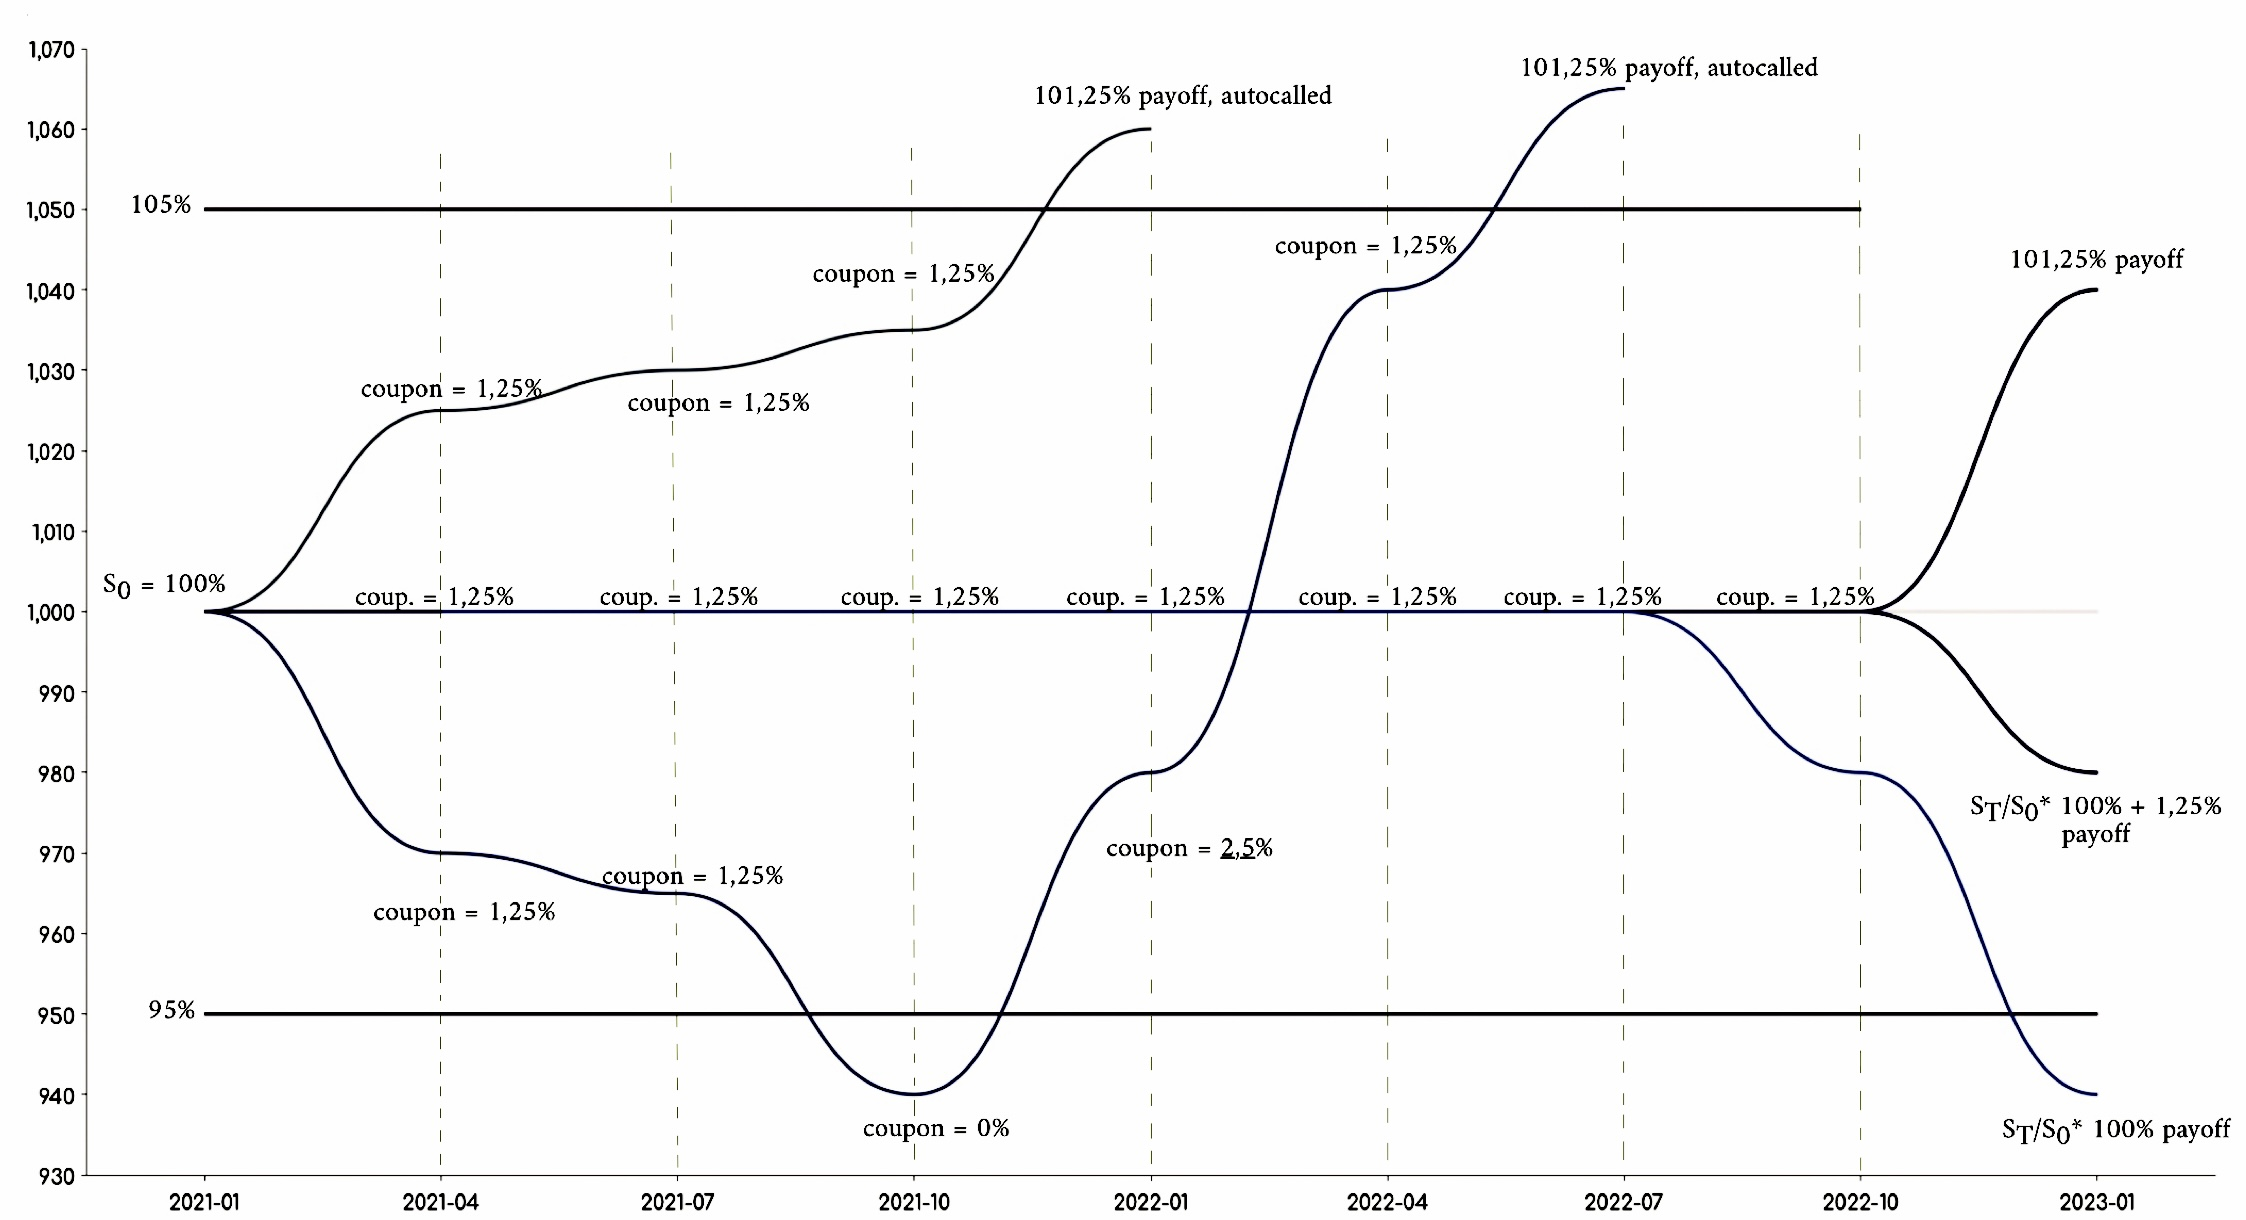
\includegraphics[width=12cm]{autocall_scheme.PNG}
\end{center}
\label{payoff}
\end{frame}


 \begin{frame}{Описание продукта}
  \begin{center}
\resizebox{10cm}{!}{
\begin{tabular}{ |c|c| } 
  \hline
    Базовые активы & Индекс «Интерфакс Российские Лидеры 1» \\ 
  \hline
    Номинал & 1000 \\
  \hline
    Срок погашения & 2 года \\
  \hline
    Автоколл барьер & 105\% \\
  \hline
    Купонный барьер & 95\% \\
  \hline
    Защитный барьер & 95\% geared put \\  
  \hline
    Купонный доход & 5\% (годовых) с эффектом памяти \\
   \hline
    Даты наблюдения & Каждые 3 месяца \\  
\end{tabular}
}
\end{center}
   \end{frame}



    \section{Модель ценообразования}
    \begin{frame}{Модель ценообразования}
    Наш продукт зависит от одного базового актива:
    \begin{align*}
        dS_t = \mu S_t dt + \sigma S_t dW_t\;, \quad S_0 = x,
    \end{align*}
    где $\mu=0,\;\sigma=10\%$.
    Обозначим даты наблюдения за $t_i$, тогда $t_{i+1}-t_i = \text{3 месяца}$ 
    \begin{align*}
        \text{Payoff}= P(S_{t_1}, ..., S_{t_n}).
    \end{align*}

    В риск-нейтральной мере цена дериватива с функцией выплат $P$, зависящей от значений базового актива $S_{t_1}, ..., S_{t_n}$, вычисляется по формуле
    \begin{align*}\label{AutocallValue}
        A(x) = \E[P(S_{t_1}, ..., S_{t_n})\; |\; S_{t_0} = x].
    \end{align*}
    \end{frame}

    \begin{frame}
    Для вычисления цены используется метод Монте--Карло. Для этого, симулируем траектории цены базового актива:
    \begin{align*}
        S_{t_i} = S_{t_{i-1}} \exp\Big((r-\frac{\sigma^2}{2})dt + \sigma \sqrt{dt} \;\epsilon_i\Big), \quad i=1,..., n, \quad S_{t_0} = x
    \end{align*}
    где $\epsilon_i$ -- н.о.р.с.в. со стандартным нормальным распределением. В данной работе было проведено сравнение между псевдослучайными и квазислучайными числами.
    \end{frame}


    \subsection{Квазислучайные числа}
    \begin{frame}{Квазислучайные числа}
        Иcкомое матожидание можно представить следующим образом: 
    \begin{align*}
        \E[P(S_{t_1}, ..., S_{t_n})\;|\; S_{t_0} = x]
        &= \E [P_1(\epsilon_1, ..., \epsilon_n)]\\
        &= \E [P_1(\Phi^{-1}(\gamma_1), ..., \Phi^{-1}(\gamma_n))]
        &= \int_{[0,1]^n} P_2(y_1, ..., y_n)\; dy,
    \end{align*}
    где $\gamma_i$ -- н.о.р.с.в. с равномерным на $[0,1]$ распределением.
    \end{frame}
    
    

    

    \section{Дельта-хеджирование}
    \begin{frame}{Дельта-хеджирование}
        Опишем более подробно эволюцию стоимости хеджирующего портфеля $P_i$ :
    \begin{enumerate} 
      \item В момент $t_0$: $P_{0} = A(t_0, S_{t_0}) - \Delta_{0} S_{t_0}$. Продали автоколл, лонг позиция с $\Delta_{0}$ акциями. По этому остатку $P_{0}$ начисляется процент по вкладу/займу: $r\cdot P_{0}$.
      
      
      \item В момент $t_1$ нужно перейти к позиции лонг с $\Delta_{1}$ акциями, что приведет к изменению стоимости на $(\Delta_0-\Delta_1)S_{t_1}$: $P_{1} = (1+r)P_{0} + (\Delta_0-\Delta_1)S_{t_1}$. И так далее.
    
      \item В момент $t_{N-1}$: $P_{N-1} = (1+r)P_{N-2} + (\Delta_{N-2}-\Delta_{N-1})S_{t_{N-1}}$
    
      \item В момент $t_N$ продаем всю имеющуюся лонг позицию в акциях, т.е. $\Delta_{N-1}$ акций: $P_{N} = (1+r)P_{N-1} + \Delta_{N-1}S_{t_{N}}$
    \end{enumerate}
    Таким образом, ошибка хеджирования высчитывается как $P_N-\text{Payoff}$.   
    \end{frame}

    \subsection{Методы вычисления дельты}
    \begin{frame}{Методы вычисления дельты}
        Cтандартный \textit{метод конечных разностей} из теории численного дифференцирования:
    
    \begin{align*}
        \Delta_S = \frac{\partial A}{\partial S} \approx \frac{A(S+\epsilon)-A(S-\epsilon)}{2\epsilon}.
    \end{align*}

        \textit{Метод коэффициента правдоподобия} дифференцирует плотность вероятности цен активов под матожиданием, что приводит к 
    \begin{align*}
        \Delta_x =  \E\Big[P(S_{t_1}, ..., S_{t_n}) \frac{Z_1}{x\sigma\sqrt{t_1-t_0}}\Big],
    \end{align*}
    где $Z_1$ -- стандартная нормальная случайная величина, использованная для генерации $S_{t_1}$ из $S_{t_0}$.     
    
    Матожидания в обоих методах будем вычислять методом Монте--Карло на псевдослучайных и квазислучайных числах.
    \end{frame}





































    
    
    \section{Практическое применение: индекс «Интерфакс Российские Лидеры 1»}
    \begin{frame}{Практическое применение}
        \begin{figure}[h!]
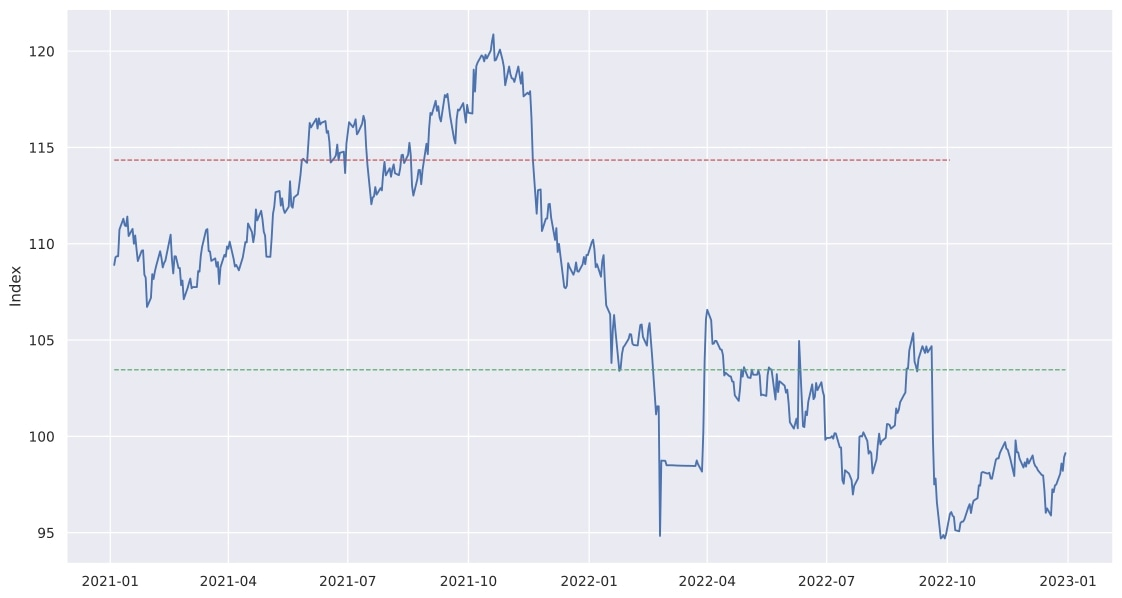
\includegraphics[width=10cm]{01.jpg} \\ Значения индекса «Интерфакс Российские Лидеры 1»
\end{figure}
 $\bullet$ Красной пунктирной линией обозначен барьер досрочного погашения, зеленым цветом - защитный барьер.

    \end{frame} 

\begin{figure}
\centering
\ \ \ \ 

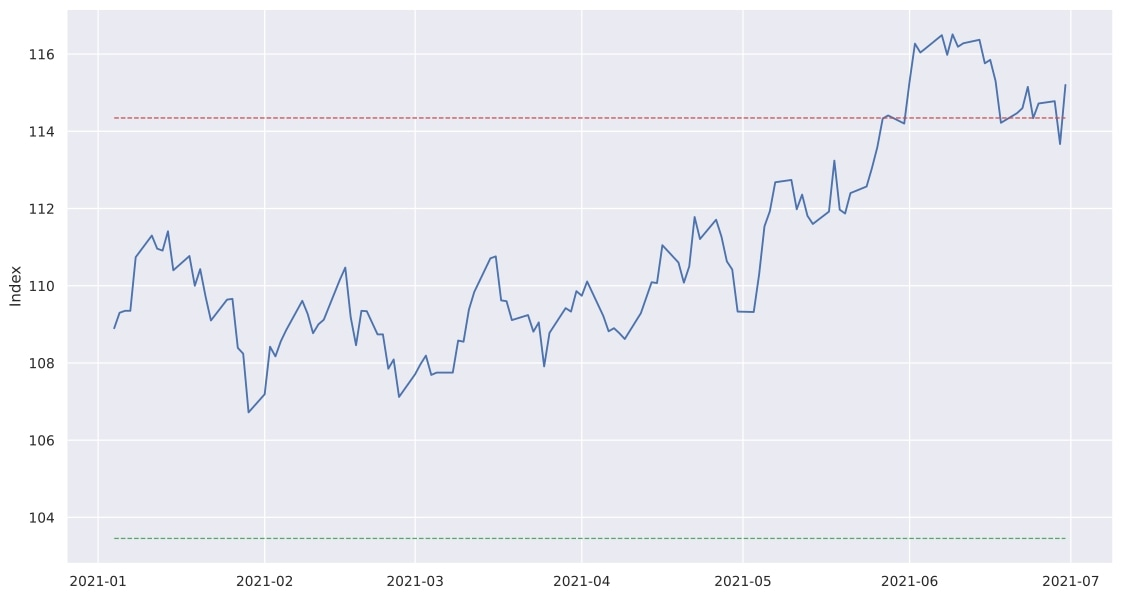
\includegraphics[width=13cm]{02.jpg} \\ Значения первых шести месяцев индекса  «Интерфакс Российские Лидеры 1»

\end{figure}

 \begin{frame}{Графики параметров индекса «Российские Лидеры 1»}
Обозначения, используемые в графиках:

 \ \ \ \ \_ps - псевдослучайные числа (pseudo-random),

 \ \ \ \ \_qs - квазислучайные числа (quasi-random),

 \ \ \ \ \_fd - метод конечных разностей (finite difference),

 \ \ \ \ \_lr - метод коэффициента правдоподобия ( likelihood ratio).
 
\

На слайдах графики будут продемонстрированы в следующем формате: слева -- результаты, полученные при использованиии псевдослучайных чисел, справа -- квазислучайных чисел.
\end{frame} 


 \begin{frame}{Стоимость Автоколла Феникс на индекс \\ «Российские Лидеры 1»}
\begin{figure}[h!]
\begin{minipage}[h!]{0.49\linewidth}
\center{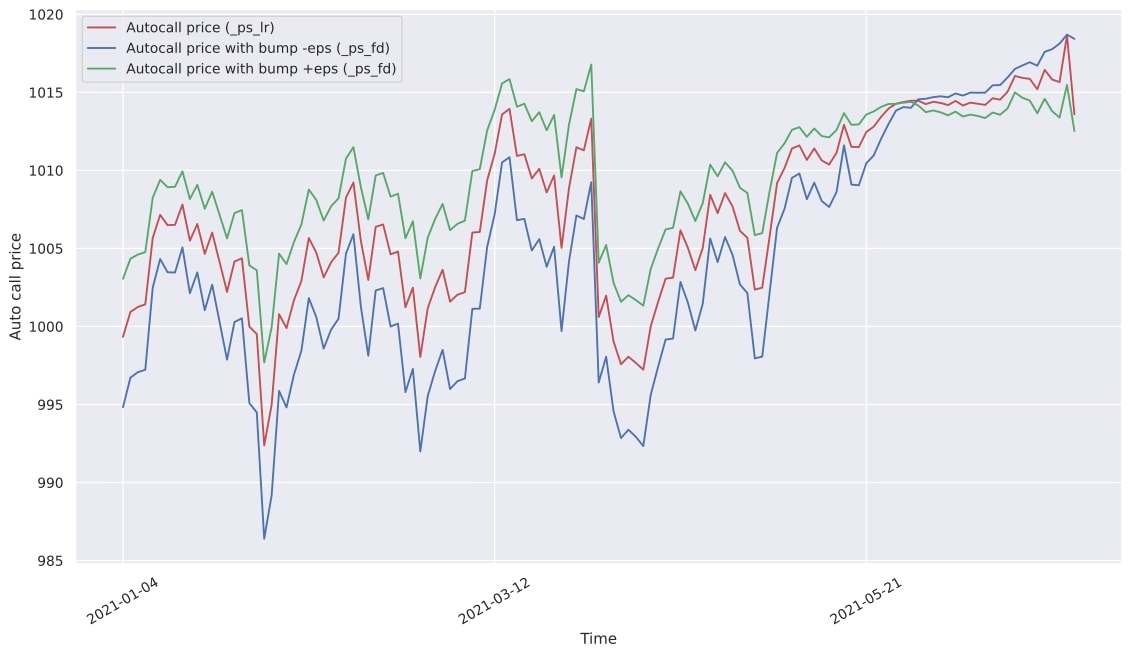
\includegraphics[width=1.08\linewidth]{03.jpg} }
\end{minipage}
\hfill
\begin{minipage}[h!]{0.49\linewidth}
\center{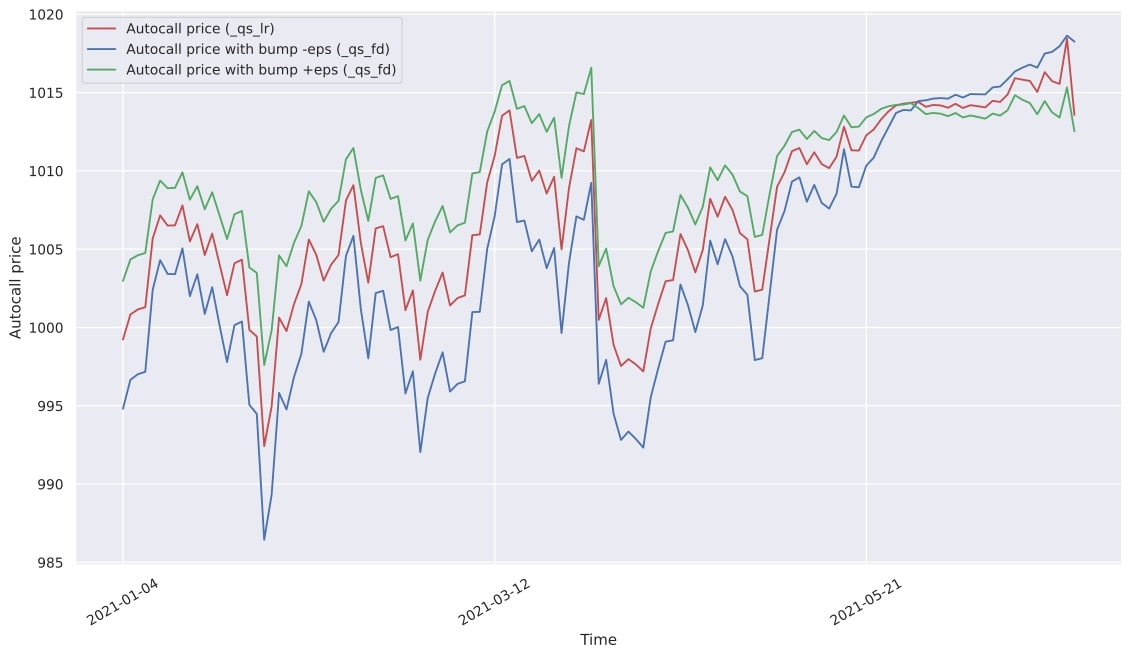
\includegraphics[width=1.08\linewidth]{04.jpg} }
\end{minipage}

\label{ris:image1}
\end{figure}
 \end{frame} 

 

 \begin{frame}{Значения дельт в каждый исторический \\ день работы Автоколла}
\begin{figure}[h]
\begin{minipage}[h]{0.49\linewidth}
\center{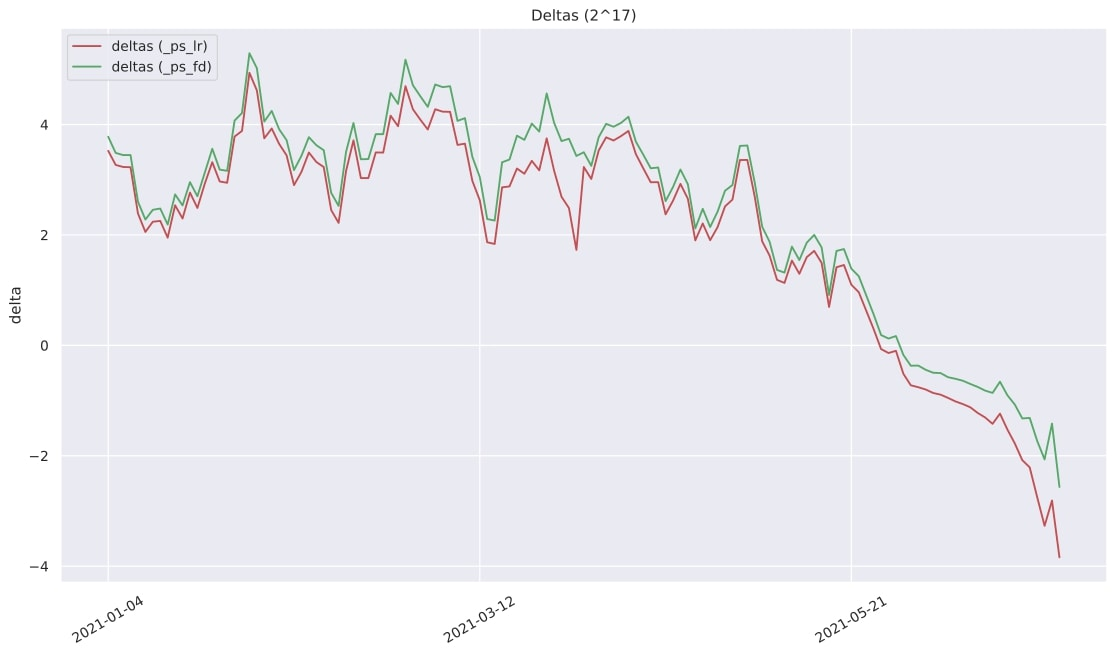
\includegraphics[width=1.08\linewidth]{05.jpg} }
\end{minipage}
\hfill
\begin{minipage}[h]{0.49\linewidth}
\center{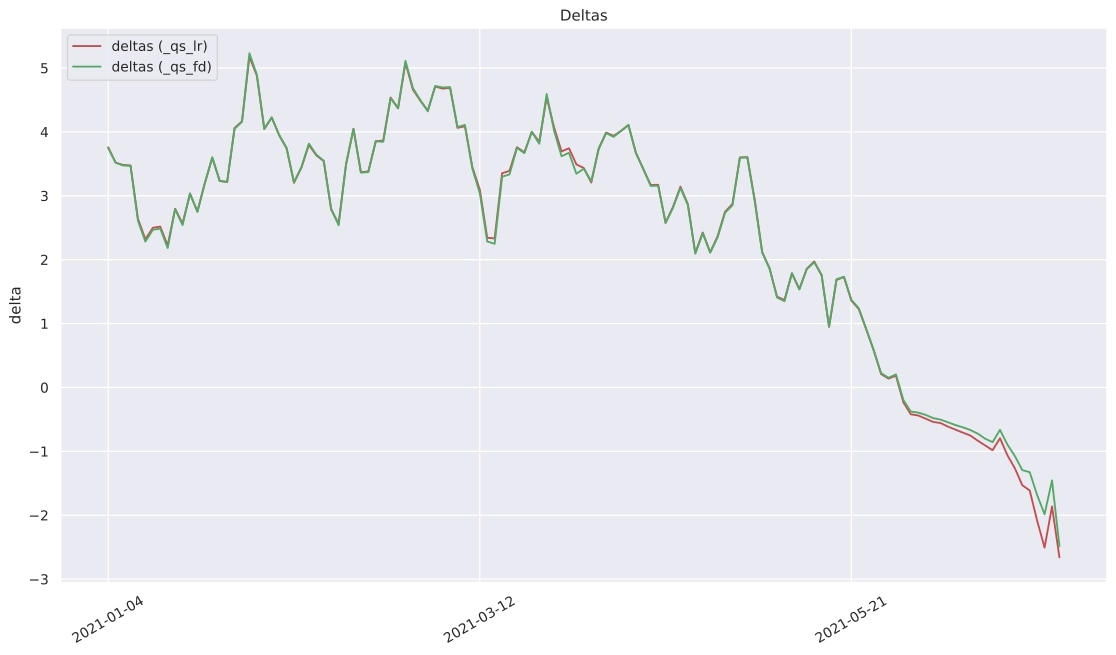
\includegraphics[width=1.08\linewidth]{06.jpg} }
\end{minipage}

\label{ris:image1}
\end{figure}


 \end{frame} 
\begin{frame}{Результаты подсчета ошибки хеджирования}
\begin{figure}[h!]
    {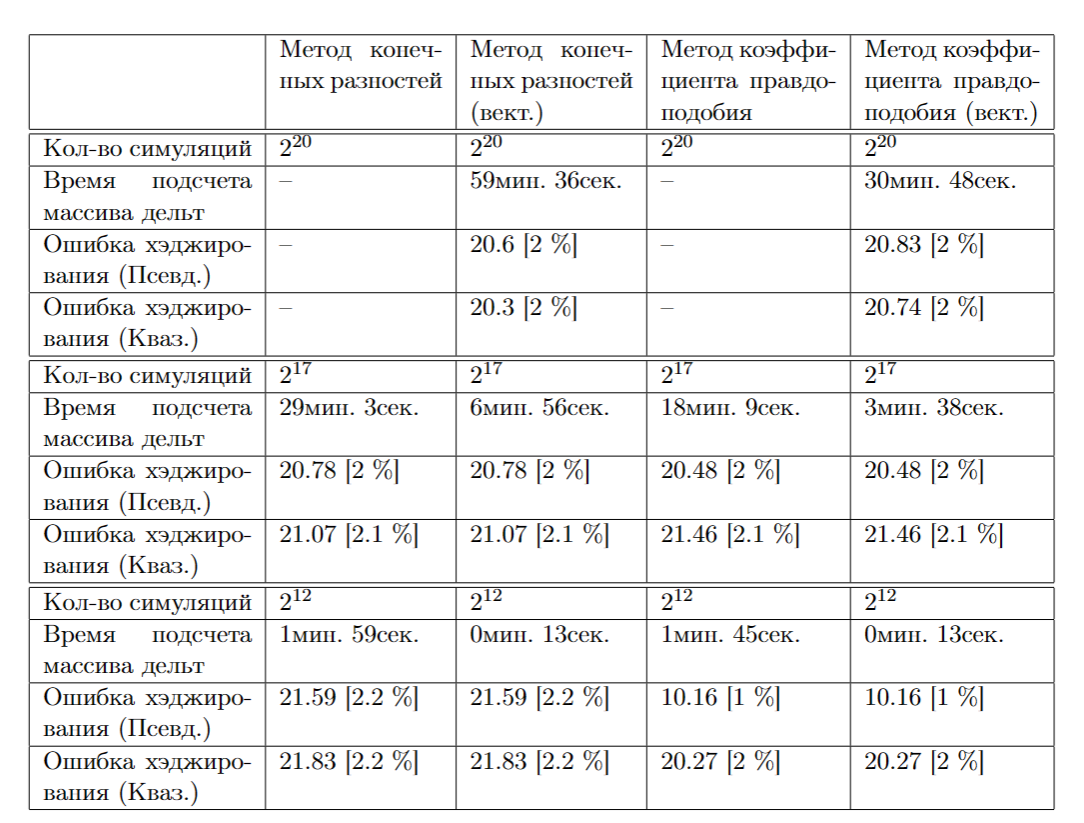
\includegraphics[width=9.2cm]{015.png}}
\end{figure}

\end{frame}

 \begin{frame}{Сходимость дельты в первый день работы \\ Автоколла Феникс на разных случайных числах}
\begin{figure}[h!]
\begin{minipage}[h!]{0.49\linewidth}
\center{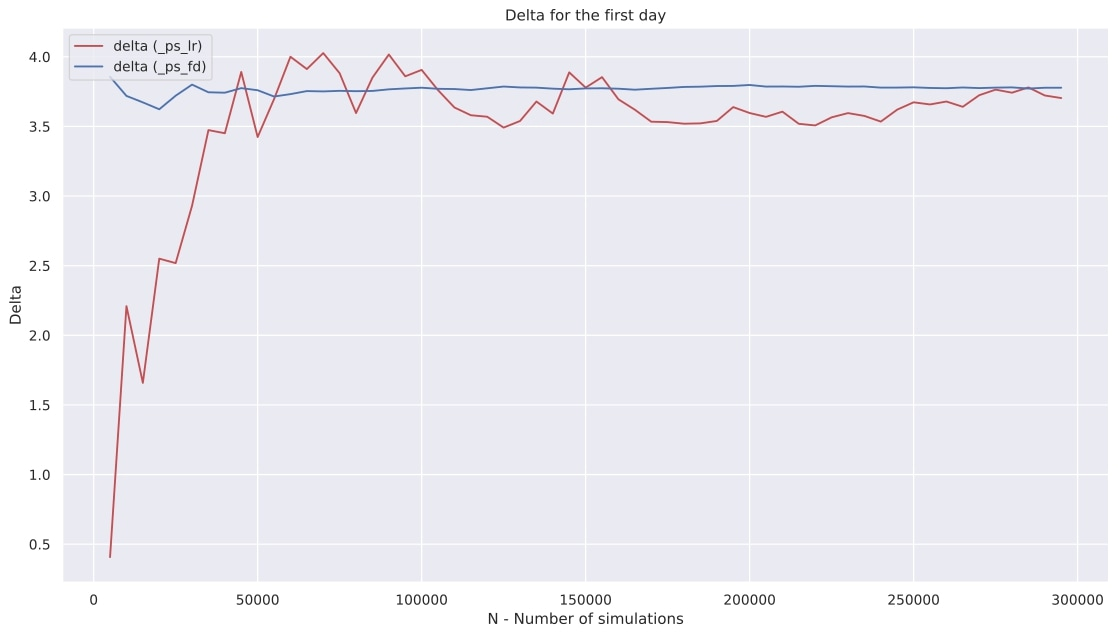
\includegraphics[width=1.08\linewidth]{07.jpg} }
\end{minipage}
\hfill
\begin{minipage}[h!]{0.49\linewidth}
\center{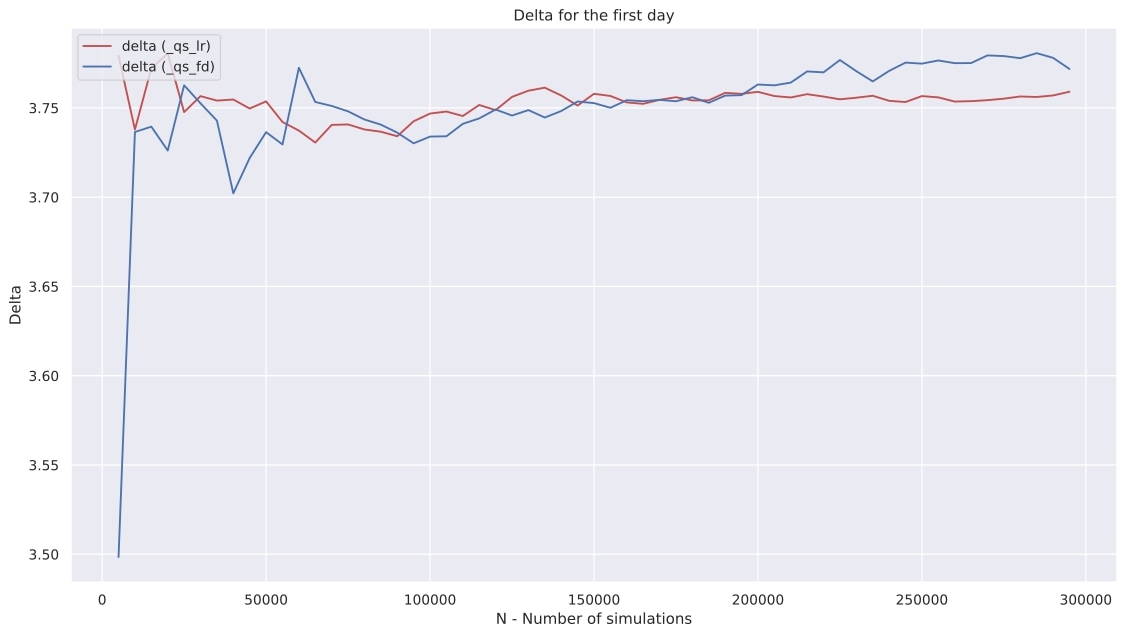
\includegraphics[width=1.08\linewidth]{08.jpg} }
\end{minipage}

\label{ris:image1}
\end{figure}
 \end{frame} 

  \begin{frame}{Сходимость дельты в первый день работы \\ Автоколла Феникс разными методами подсчета}
\begin{figure}[h!]
\begin{minipage}[h!]{0.49\linewidth}
\center{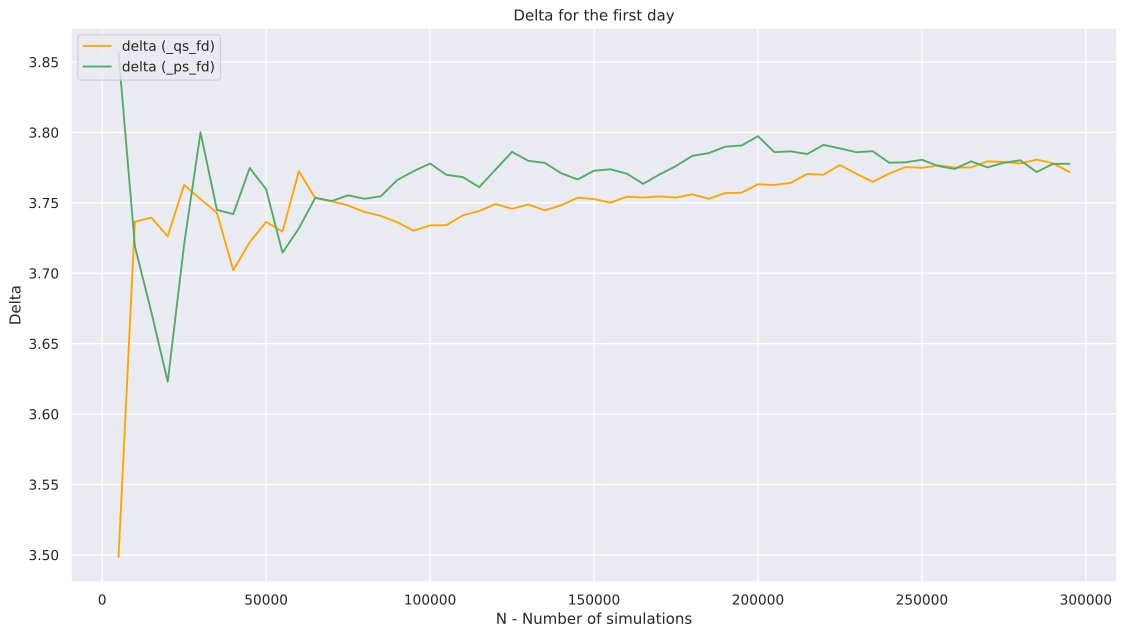
\includegraphics[width=1.08\linewidth]{011.jpg} }
\end{minipage}
\hfill
\begin{minipage}[h!]{0.49\linewidth}
\center{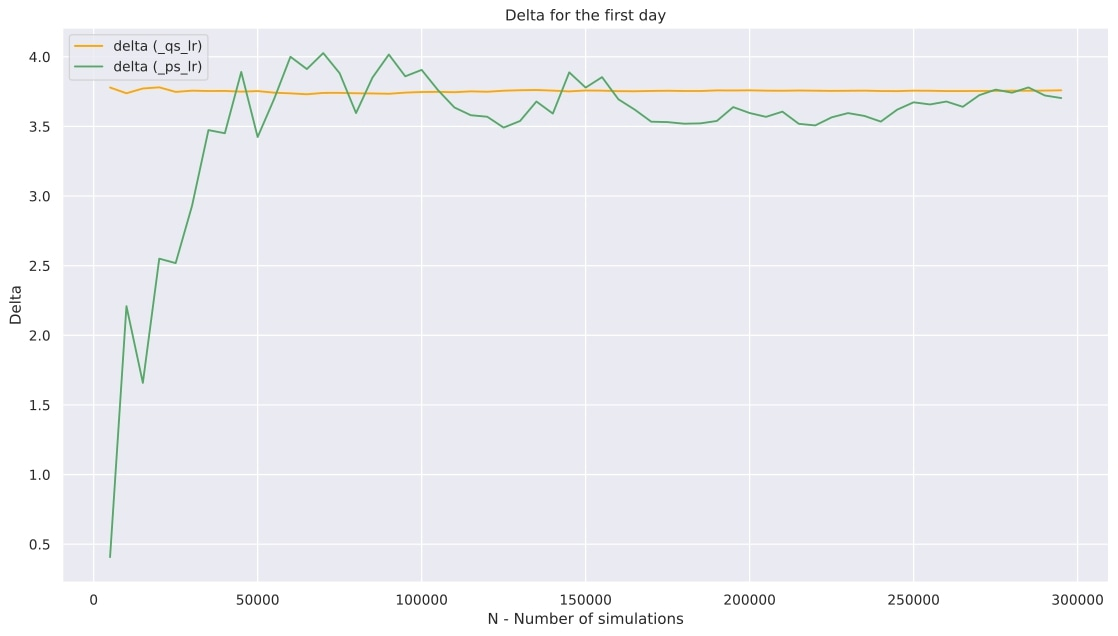
\includegraphics[width=1.08\linewidth]{012.jpg} }
\end{minipage}

\label{ris:image1}
\end{figure}
 \end{frame} 

 
    \section{Заключение}
    \begin{frame}{Заключение}
         В данной работе были проведены вычислительные эксперименты, указывающие на состоятельность данных методов. Анализируя графики сходимости дельты, можно построить следующую схему: 
\begin{center}
    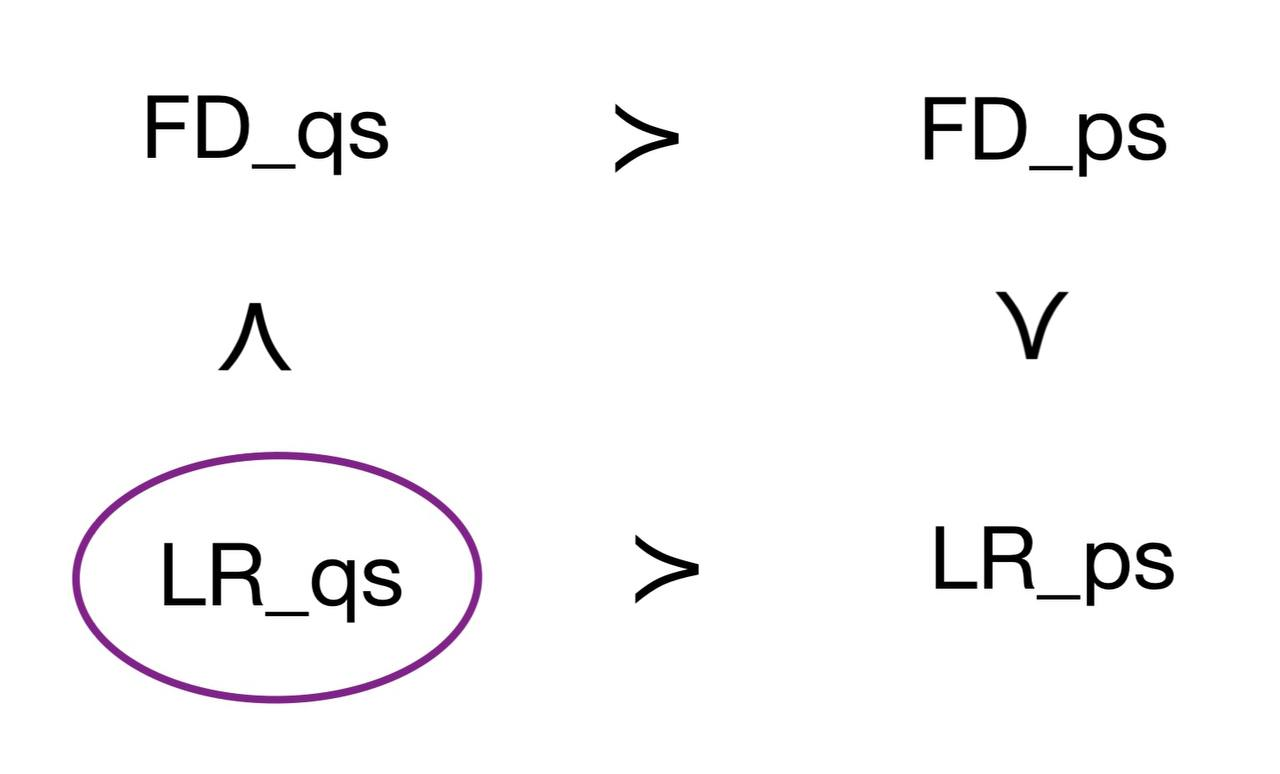
\includegraphics[width=.5\linewidth]{methods.jpg} 
\end{center}

Выходит, что из всех четырех случаев предпочтительнее использовать метод \textit{LR на квазислучайных последовательностях}.

    \end{frame}
    \section{Литература}
    \begin{frame}{Литература}
    
%    \nocite{*} % Insert publications even if they are not cited in the poster
    \nocite{*}
    \printbibliography
   
    \end{frame}


 
\end{document}